\chapter{Validation}
\label{chap:validation}

\vspace{-\baselineskip}

%##################################################################################################
\section{Chapter Overview}
%##################################################################################################

In order to evaluate the effectiveness of my approach, I undertook two separate pieces of validation work. The first piece involved quantifying the accuracy of the 3D feature identifiers presented in the previous chapter -- this was done by comparing their output to `gold standard' results produced manually in collaboration with a radiologist. The second piece involved validating the accuracy of my volume calculations. To do this, I first manually identified the liver, kidneys and spleen in a number of series and used my program to calculate their volumes in each case. The volume results were then correlated with known weights provided by the radiologist (bearing in mind that the densities of the organs in question are relatively uniform).

Both producing the gold standard results and making inter-result comparisons involved implementing special features for the purpose in \emph{millipede}. For the gold standard production, manual drawing tools were implemented to allow the user to draw round features of interest in the images. To make life easier for the user, the actual drawing was done using a \emph{Bamboo Fun} pen tablet (manufactured by Wacom) -- see Figure~\ref{fig:validation-pentablet-usage} -- although it would also have been possible to use a standard mouse. The inter-result comparisons were implemented as a dialog box allowing the user to compare multi-feature selections on a per-feature basis. The implementation of all the validation-specific features is discussed in Appendix~\ref{chap:appendixval}.

The validation work undertaken here forms an important part of the basis for the following chapter, in which I critically assess all the contributions claimed in the introduction.

%---
\stufigex{height=20cm}{validation/validation-pentablet-usage.png}{A typical user drawing round the right kidney using a `lasso' drawing tool similar to that found in common image-editing programs}{fig:validation-pentablet-usage}{p}
%---

%##################################################################################################
\section{Validation of Feature Identifiers}
%##################################################################################################

TODO

%################################################
\subsection{Series BT-2, Slices $60$--$80$}
%################################################

TODO

\begin{center}
\begin{tabular}{cccccccc}
\scriptsize \textbf{Feature} & \scriptsize \textbf{Target} & \scriptsize \textbf{Gold} & \scriptsize \textbf{T - G} & \scriptsize \textbf{G - T} & \scriptsize \textbf{T $\cap$ G} & \scriptsize \textbf{Dice} & \scriptsize \textbf{Jaccard} \\
\hline
\scriptsize Aorta & \scriptsize 13940 & \scriptsize 13973 & \scriptsize 1949 & \scriptsize 1982 & \scriptsize 11991 & \scriptsize 0.859 & \scriptsize 0.753 \\
\scriptsize Kidney & \scriptsize 72142 & \scriptsize 73715 & \scriptsize 2915 & \scriptsize 4488 & \scriptsize 69227 & \scriptsize 0.949 & \scriptsize 0.903 \\
\scriptsize Liver & \scriptsize 180156 & \scriptsize 180693 & \scriptsize 19624 & \scriptsize 20161 & \scriptsize 160532 & \scriptsize 0.890 & \scriptsize 0.801 \\
\scriptsize Rib & \scriptsize 22787 & \scriptsize 31125 & \scriptsize 1942 & \scriptsize 10280 & \scriptsize 20845 & \scriptsize 0.773 & \scriptsize 0.630 \\
\scriptsize Spinal Canal & \scriptsize 14451 & \scriptsize 11002 & \scriptsize 3758 & \scriptsize 309 & \scriptsize 10693 & \scriptsize 0.840 & \scriptsize 0.724 \\
\scriptsize Spleen & \scriptsize 11841 & \scriptsize 15077 & \scriptsize 359 & \scriptsize 3595 & \scriptsize 11482 & \scriptsize 0.853 & \scriptsize 0.744 \\
\scriptsize Vertebra & \scriptsize 111889 & \scriptsize 113385 & \scriptsize 7634 & \scriptsize 9130 & \scriptsize 104255 & \scriptsize 0.926 & \scriptsize 0.861 \\
\end{tabular}
\end{center}

%---
\begin{stusubfig}{p}
	\subfigure[Gold Standard Result]
	{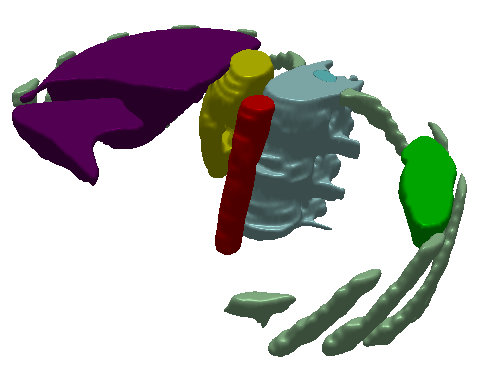
\includegraphics[width=.45\linewidth]{validation/validation-BT-2-60-80-goldstandard.png}}%
	%
	\hspace{4mm}%
	%
	\subfigure[Automated Result]
	{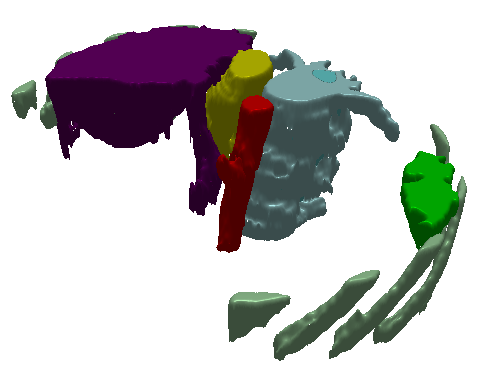
\includegraphics[width=.45\linewidth]{validation/validation-BT-2-60-80-target.png}}%
\caption{A comparison of the gold standard and automated results for the BT-2-60-80 feature identification case study}
\label{fig:validation-BT-2-60-80}
\end{stusubfig}
%---

%################################################
\subsection{Series SD-2, Slices $70$--$90$}
%################################################

TODO

\begin{center}
\begin{tabular}{cccccccc}
\scriptsize \textbf{Feature} & \scriptsize \textbf{Target} & \scriptsize \textbf{Gold} & \scriptsize \textbf{T - G} & \scriptsize \textbf{G - T} & \scriptsize \textbf{T $\cap$ G} & \scriptsize \textbf{Dice} & \scriptsize \textbf{Jaccard} \\
\hline
\scriptsize Aorta & \scriptsize 12799 & \scriptsize 9848 & \scriptsize 3619 & \scriptsize 668 & \scriptsize 9180 & \scriptsize 0.811 & \scriptsize 0.682 \\
\scriptsize Kidney & \scriptsize 93853 & \scriptsize 91324 & \scriptsize 7671 & \scriptsize 5142 & \scriptsize 86182 & \scriptsize 0.931 & \scriptsize 0.871 \\
\scriptsize Liver & \scriptsize 254945 & \scriptsize 231766 & \scriptsize 28156 & \scriptsize 4977 & \scriptsize 226789 & \scriptsize 0.932 & \scriptsize 0.873 \\
\scriptsize Rib & \scriptsize 10331 & \scriptsize 10097 & \scriptsize 1962 & \scriptsize 1728 & \scriptsize 8369 & \scriptsize 0.819 & \scriptsize 0.694 \\
\scriptsize Spinal Canal & \scriptsize 15163 & \scriptsize 11655 & \scriptsize 3609 & \scriptsize 101 & \scriptsize 11554 & \scriptsize 0.862 & \scriptsize 0.757 \\
\scriptsize Spleen & \scriptsize 46129 & \scriptsize 55049 & \scriptsize 1922 & \scriptsize 10842 & \scriptsize 44207 & \scriptsize 0.874 & \scriptsize 0.776 \\
\scriptsize Vertebra & \scriptsize 84757 & \scriptsize 85430 & \scriptsize 2624 & \scriptsize 3297 & \scriptsize 82133 & \scriptsize 0.965 & \scriptsize 0.933 \\
\end{tabular}
\end{center}

%---
\begin{stusubfig}{p}
	\subfigure[Gold Standard Result]
	{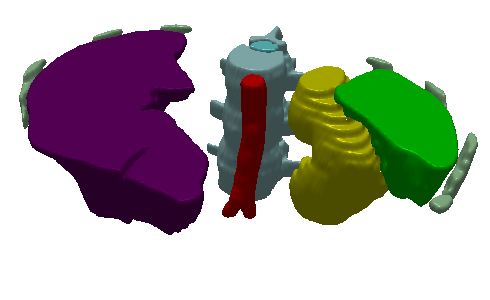
\includegraphics[width=.45\linewidth]{validation/validation-SD-2-70-90-goldstandard.png}}%
	%
	\hspace{4mm}%
	%
	\subfigure[Automated Result]
	{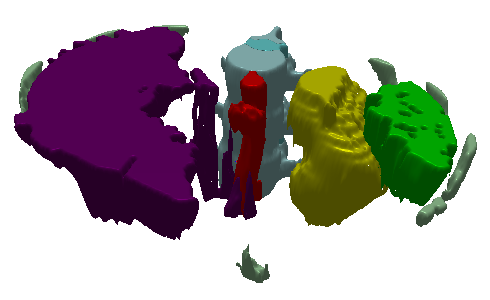
\includegraphics[width=.45\linewidth]{validation/validation-SD-2-70-90-target.png}}%
\caption{A comparison of the gold standard and automated results for the SD-2-70-90 feature identification case study}
\label{fig:validation-SD-2-70-90}
\end{stusubfig}
%---

%################################################
\subsection{Series MC-2, Slices $110$--$130$}
%################################################

TODO

\begin{center}
\begin{tabular}{cccccccc}
\scriptsize \textbf{Feature} & \scriptsize \textbf{Target} & \scriptsize \textbf{Gold} & \scriptsize \textbf{T - G} & \scriptsize \textbf{G - T} & \scriptsize \textbf{T $\cap$ G} & \scriptsize \textbf{Dice} & \scriptsize \textbf{Jaccard} \\
\hline
\scriptsize Aorta & \scriptsize 15799 & \scriptsize 15036 & \scriptsize 1805 & \scriptsize 1042 & \scriptsize 13994 & \scriptsize 0.908 & \scriptsize 0.831 \\
\scriptsize Kidney & \scriptsize 148065 & \scriptsize 137416 & \scriptsize 18698 & \scriptsize 8049 & \scriptsize 129367 & \scriptsize 0.906 & \scriptsize 0.829 \\
\scriptsize Liver & \scriptsize 492435 & \scriptsize 413475 & \scriptsize 108454 & \scriptsize 29494 & \scriptsize 383981 & \scriptsize 0.848 & \scriptsize 0.736 \\
\scriptsize Rib & \scriptsize 33626 & \scriptsize 42708 & \scriptsize 2483 & \scriptsize 11565 & \scriptsize 31143 & \scriptsize 0.816 & \scriptsize 0.689 \\
\scriptsize Spinal Canal & \scriptsize 9924 & \scriptsize 9087 & \scriptsize 1054 & \scriptsize 217 & \scriptsize 8870 & \scriptsize 0.933 & \scriptsize 0.875 \\
\scriptsize Spleen & \scriptsize 32048 & \scriptsize 36537 & \scriptsize 1240 & \scriptsize 5729 & \scriptsize 30808 & \scriptsize 0.898 & \scriptsize 0.816 \\
\scriptsize Vertebra & \scriptsize 81483 & \scriptsize 79453 & \scriptsize 5247 & \scriptsize 3217 & \scriptsize 76236 & \scriptsize 0.947 & \scriptsize 0.900 \\
\end{tabular}
\end{center}

%---
\begin{stusubfig}{p}
	\subfigure[Gold Standard Result]
	{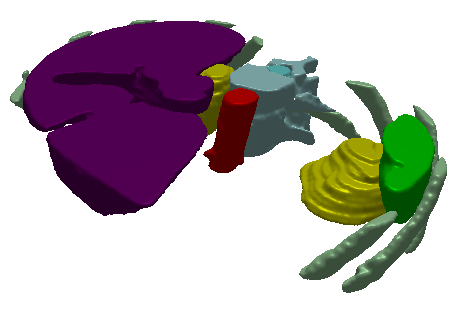
\includegraphics[width=.45\linewidth]{validation/validation-MC-2-110-130-goldstandard.png}}%
	%
	\hspace{4mm}%
	%
	\subfigure[Automated Result]
	{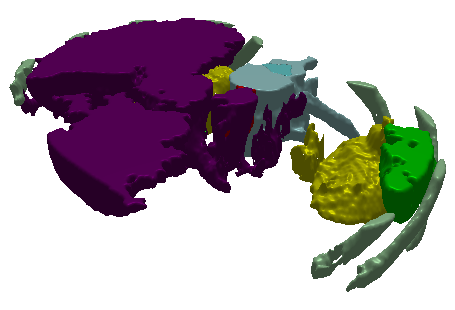
\includegraphics[width=.45\linewidth]{validation/validation-MC-2-110-130-target.png}}%
	%
	\hspace{4mm}%
	%
	\subfigure[Automated Result (excluding liver)]
	{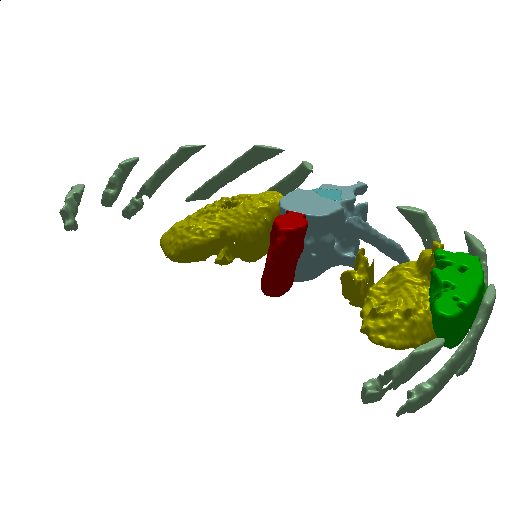
\includegraphics[width=.45\linewidth]{validation/validation-MC-2-110-130-target-noliver.png}}%
\caption{TODO}
\label{fig:validation-MC-2-110-130}
\end{stusubfig}
%---

%################################################
\subsection{Series EB-2, Slices $60$--$80$}
%################################################

TODO (the left kidney is missed due to a tumour; the spleen is missed because there's not enough of it in the slices chosen (check this); the ribs are oversegmented because there are lots of unusually bright non-rib bits in EB-2)

\begin{center}
\begin{tabular}{cccccccc}
\scriptsize \textbf{Feature} & \scriptsize \textbf{Target} & \scriptsize \textbf{Gold} & \scriptsize \textbf{T - G} & \scriptsize \textbf{G - T} & \scriptsize \textbf{T $\cap$ G} & \scriptsize \textbf{Dice} & \scriptsize \textbf{Jaccard} \\
\hline
\scriptsize Aorta & \scriptsize 10365 & \scriptsize 9416 & \scriptsize 1969 & \scriptsize 1020 & \scriptsize 8396 & \scriptsize 0.849 & \scriptsize 0.737 \\
\scriptsize Kidney (Right) & \scriptsize 47444 & \scriptsize 46918 & \scriptsize 3461 & \scriptsize 2935 & \scriptsize 43983 & \scriptsize 0.932 & \scriptsize 0.873 \\
\scriptsize Kidney (Left) & \scriptsize 0 & \scriptsize 36874 & \scriptsize 0 & \scriptsize 36874 & \scriptsize 0 & \scriptsize 0.000 & \scriptsize 0.000 \\
\scriptsize Liver & \scriptsize 160978 & \scriptsize 164834 & \scriptsize 6592 & \scriptsize 10448 & \scriptsize 154386 & \scriptsize 0.948 & \scriptsize 0.901 \\
\scriptsize Rib & \scriptsize 10256 & \scriptsize 4959 & \scriptsize 6542 & \scriptsize 1245 & \scriptsize 3714 & \scriptsize 0.488 & \scriptsize 0.323 \\
\scriptsize Spinal Canal & \scriptsize 12387 & \scriptsize 9645 & \scriptsize 2958 & \scriptsize 216 & \scriptsize 9429 & \scriptsize 0.856 & \scriptsize 0.748 \\
\scriptsize Spleen & \scriptsize 0 & \scriptsize 20179 & \scriptsize 0 & \scriptsize 20179 & \scriptsize 0 & \scriptsize 0.000 & \scriptsize 0.000 \\
\scriptsize Vertebra & \scriptsize 82721 & \scriptsize 85490 & \scriptsize 4946 & \scriptsize 7715 & \scriptsize 77775 & \scriptsize 0.925 & \scriptsize 0.860 \\
\end{tabular}
\end{center}

%---
\begin{stusubfig}{p}
	\subfigure[Gold Standard Result]
	{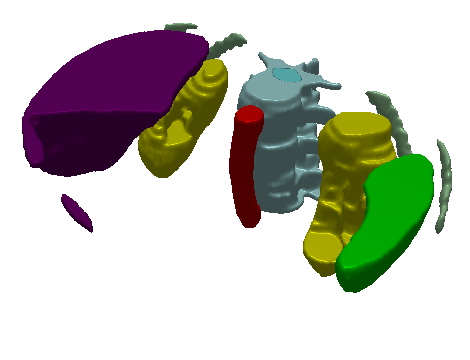
\includegraphics[width=.45\linewidth]{validation/validation-EB-2-60-80-goldstandard.png}}%
	%
	\hspace{4mm}%
	%
	\subfigure[Automated Result]
	{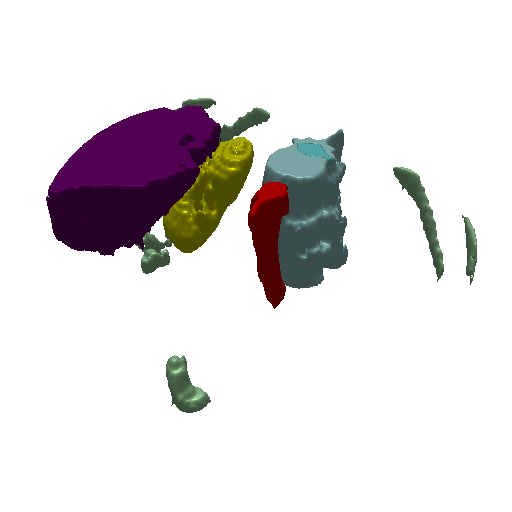
\includegraphics[width=.45\linewidth]{validation/validation-EB-2-60-80-target.png}}%
\caption{A comparison of the gold standard and automated results for the EB-2-60-80 feature identification case study}
\label{fig:validation-EB-2-60-80}
\end{stusubfig}
%---

\afterpage{\clearpage}
\newpage

%##################################################################################################
\section{Validation of Volume Calculations}
%##################################################################################################

TODO: \cite{woodard86}

%---
\begin{landscape}
\begin{figure}[p]
\footnotesize
\begin{center}
\begin{tabular}{c|rrc|rrc|rr|rr}
\textbf{Patient} & \multicolumn{3}{|c|}{\textbf{Left Kidney}} & \multicolumn{3}{|c|}{\textbf{Right Kidney}} & \multicolumn{2}{|c|}{\textbf{Liver}} & \multicolumn{2}{|c}{\textbf{Spleen}} \\
& \emph{Mass} ($g$) & \emph{Vol.} ($\mathit{cm}^3$) & \emph{Cysts} $> 5\mathit{mm}$ & \emph{Mass} ($g$) & \emph{Vol.} ($\mathit{cm}^3$) & \emph{Cysts} $> 5\mathit{mm}$ & \emph{Mass} ($g$) & \emph{Vol.} ($\mathit{cm}^3$) & \emph{Mass} ($g$) & \emph{Vol.} ($\mathit{cm}^3$) \\
\hline
\hline
OX25 & 120 &  96.116 &            --- & 110 &  96.044 &                            --- & 1680 & 1468.657 & 110 & 105.568 \\
OX26 & 190 & 173.155 &            --- & 190 & 175.411 &                            --- & 1790 & 1752.384 &  40 &  32.879 \\
OX27 &  80 &  74.897 &              6 &  85 &  84.300 &                             12 & 1370 & 1156.192 & 140 & 121.837 \\
OX29 & 110 & 106.566 &            --- &  90 &  94.306 &                            --- & 1380 & 1323.991 & 170 & 121.665 \\
OX30 & 120 & 126.524 &         28, 27 & 120 & 113.079 &                              9 & 1819 & 1662.805 & 180 & 158.506 \\
OX31 & 200 & 175.163 &             14 & 170 & 153.155 &                            --- & 2120 & 1972.002 & 110 &  98.132 \\
OX33 & 120 & 111.776 &         12, 10 & 110 & 105.223 &                             10 & 1010 & 1042.976 & 110 &  98.362 \\
OX34 & 100 &  91.514 &            --- & 110 &  93.505 &                            --- &  880 &  792.150 &  70 &  65.271 \\
OX35 &  95 &  93.405 &             32 &  90 &  81.308 &                            --- & 1120 & 1091.544 &  45 &  35.542 \\
OX36 & 170 & 147.269 & 25, 19, 17, 10 & 140 & 126.720 & 15 ($\times$4), 10 ($\times$2) & 1660 & 1410.233 & 260 & 237.772 \\
OX37 & 160 & 132.421 &             23 & 140 & 110.786 &                            --- & 1210 & 1016.613 & 120 &  91.921 \\
OX38 & 126 & 114.638 & 24, 18, 13, 12 & 134 & 112.267 &                            --- & 1387 & 1501.876 & 196 & 203.940 \\
OX39 & 125 & 105.321 &            --- & 120 & 113.161 &                            --- & 1250 & 1212.430 & 120 & 104.221 \\
OX40 & 140 & 121.521 &            --- & 140 & 117.883 &                            --- & 1390 & 1297.704 & 110 &  78.971 \\
OX41 & 150 & 110.221 &            --- & 120 &  94.978 &                            --- & 1670 & 1577.043 & 150 & 124.464 \\
OX42 & 230 & 183.583 &            --- & 180 & 160.707 &                            --- & 1650 & 1565.364 & 100 &  85.891 \\
OX43 & 140 & 111.631 &            --- & 150 & 124.826 &                            --- & 1200 & 1066.671 & 190 & 165.091 \\
OX44 & 140 & 111.968 &            --- & 130 & 112.832 &                            --- & 1440 & 1344.238 & 130 &  83.531 \\
OX46 & 130 & 115.295 &            --- & 130 & 303.460 &                             80 & 1000 & 1020.945 &  90 &  81.773
\end{tabular}
\end{center}
\caption{TODO}
\label{fig:validation-volcalc-table}
\end{figure}
\end{landscape}
%---

%---
\stufigex{height=9cm}{validation/validation-volcalc-leftkidney.png}{TODO}{fig:validation-volcalc-leftkidney}{p}
%---

%---
\stufigex{height=9cm}{validation/validation-volcalc-rightkidney.png}{TODO}{fig:validation-volcalc-rightkidney}{p}
%---

%---
\stufigex{height=9cm}{validation/validation-volcalc-liver.png}{TODO}{fig:validation-volcalc-liver}{p}
%---

%---
\stufigex{height=9cm}{validation/validation-volcalc-spleen.png}{TODO}{fig:validation-volcalc-spleen}{p}
%---

%##################################################################################################
\section{Chapter Summary}
%##################################################################################################

TODO
